% \documentclass[11pt,letterpaper]{article}
\documentclass[twocolumn]{article}
\usepackage[utf8]{inputenc}
\usepackage{epsfig,graphicx}
\usepackage[left=2cm,right=2cm,top=1.8cm,bottom=2.3cm]{geometry}
\usepackage{fancyhdr}
\usepackage{fancyvrb}
\usepackage{lastpage}
\usepackage{movie15}
\usepackage[demo]{graphicx}
\usepackage{subfig}
\fancyhf{}
\usepackage{amsmath}
\usepackage{amssymb}
\usepackage{amsthm}
\usepackage{lipsum}
\usepackage{cuted}
\usepackage[font=small,skip=0pt]{caption}

\usepackage{pgfplots}
\pgfplotsset{width=8cm,compat=1.9}
\usepgfplotslibrary{external}
\tikzexternalize

\begin{document}
\begin{strip}
\begin{tightcenter}
\rule{17.5cm}{0.1mm}\\[5mm]
    \begin{minipage}{3cm}
    	\begin{center}
    		\includegraphics[height=3.4cm]{pw_logo.jpg}
    	\end{center}
    \end{minipage}\hfill
    \begin{minipage}{10cm}
    	\begin{center}
    	\textbf{\large Politechnika Warszawska}\\[0.1cm]
        \textbf{Wydzial Geodezji i Kartografii}\\[0.1cm]
        \textbf{Geoinformatyka $|$ 2023L}\\[0.1cm]
        Systemy Nawigacji Satelitarnej\\[0.1cm]
        Planowanie pomiarow GNSS\\[0.1cm]
        Szymon Kolakowski, 19.03.2023
    	\end{center}
    \end{minipage}\hfill
    \begin{minipage}{3cm}
    	\begin{center}
    		\includegraphics[height=3.4cm]{gik_logo.png}
    	\end{center}
    \end{minipage}\\[5mm]
\rule{17.5cm}{0.1mm}
\end{tightcenter}
\end{strip}

\section{Omowienie algorytmu obliczen}

% \subsection{Przygotowanie danych}

% Zeby myslec o wykonywaniu jakichkolwiek obliczen, program musi najpierw sparsowac plik z danymi almanachu a takze wszystkie parametry przekazane przez uzytkownika w wierszu polecen. Odpowiadaja za to funkcje umieszczone w plikach \textbf{lib/ALMtoCSV.c} oraz \textbf{lib/CMDtoARGS.c} ktorych nie warto bardziej szczegolowo tutaj omawiac, gdyz sa to jedynie standardowe operacje na strumieniach wejscia/wyjscia w jezyku C. Pliki te znaduja sie w zalacznikach do sprawozdania.

% \subsection{Transformacje jednostek}

% Korzystajac z danych otrzymanych w poprzednim etapie, program dokonuje teraz dwoch przeksztalcen ktore umozliwia rozpoczecie wykonywania obliczen. Pierwszym jest zamiana jednostki ze stopni na radiany zarowno dla miar katow zamieszczonych w almanachu jak i dla wspolrzednych odbiornika. Drugim jest transformacja dat poczatku i zakonczenia pomiarow do skali czasu GPS. Odpowiada za to funkcja umieszczona w pliku \textbf{lib/DATEtoGPSTIME.c} zwracajaca liczbe sekund ktore uplynely od poczatku dnia 06.01.1980.

\subsection{Wspolrzedne globalne satelity}

Pliki danych efemerydalnych zawieraja parametry orbit oskulacyjnych satelitow. Sa to orbity keplerowskie, styczne do orbity rzeczywistej w punkcie w ktorym satelita znajdowal sie w chwili ich wyznaczania, dokladnie odwzorowujace wektor predkosci satelity. Z uwagi na to ze parametry orbity keplerowskiej sa stale, mozemy wyznaczyc pozycje satelitow w dowolnym momencie czasu (tzw. epoce (1)).
\begin{equation}
t_k=t_{pomiaru}-t_{almanachu}
\end{equation}
Dla przyspieszenia obliczen na starszych komputerach, w almanachu podaje sie pierwiastek duzej polosi orbity. Juz na samym poczatku warto podniesc go do kwadratu aby ulatwic sobie poslugiwanie sie ta zmienna przy dalszych wzorach.
\begin{equation}
a=(\sqrt{a})^2
\end{equation}
Korzystajac z Trzeciego Prawa Keplera mozemy wyznaczyc wzor na predkosc katowa n (tzw ruch sredni)
\begin{equation}
\frac{a^3}{T^2}=\frac{\mu}{4\pi^2}\to\mu=a^3n^2\to n=\sqrt{\frac{\mu}{a^3}} 
\end{equation}
gdzie \(\mu\) to standardowy parametr grawitacyjny, staly dla konkretnego systemu grawitacyjnego. przy jego wyznaczaniu mozemy pominac mase satelity gdyz jest ona zaniedbywalna w perspektywie masy Ziemi
\begin{equation}
\mu = G(M+m) \to GM = 3.986005\cdot10^1^4[\frac{m^3}{s^2}]
\end{equation}
predkosc katowa pozwala na wyznaczenie tzw anomalii sredniej na epoke pomiaru. Anomalię średnią można sobie wyobrazić jako kąt, opisujący położenie fikcyjnego punktu poruszającego się ze stałą prędkością kątową n po okręgu opisanym na orbicie.
\begin{equation}
M_k=M_0+n\cdot t_k
\end{equation}
gdzie \(M_0\) to wartosc anomalii sredniej na epoke almanachu. korzystajac z wyznaczonej wartosci \(M_k\) oraz rownania Keplera, mozemy wyznaczyc anomalie mimosrodowa (parametr opisujący ruch ciała po orbicie keplerowskiej, zdefiniowana jako kąt pomiędzy odcinkiem łączącym geometryczny środek orbity z perycentrum a odcinkiem łączącym geometryczny środek orbity z punktem wyznaczonym przez przecięcie prostej prostopadłej do linii apsyd, przechodzącej przez ciało i okręgu opisanego na orbicie). wyliczamy jej wartosc iteracyjnie korzystajac ze wzorow (6) tak dlugo jak niespelniony pozostaje warunek (6c).
\begin{equation}
E_1=M_k
\end{equation}
\begin{equation}
E_i_+_1=M_k+e\sin{(E_i)}
\end{equation}
\begin{equation}
|E_i-E_i_-_1|<10^-^1^2
\end{equation}
wartosc anomalii mimosrodowej pozwala na wyznaczenie anomalii prawdziwej, tzn kata zawartego pomiędzy kierunkiem od ogniska orbity do perycentrum a kierunkiem od ogniska do ciała na orbicie
\begin{equation}
v_k=\arctan{\Big(\frac{\sqrt{1-e^2}\sin{(E_k)}}{\cos{(E_k)}-e}\Big)}
\end{equation}
otrzymana wartosc mozemy powiazac z argumentem perygeum (kąt pozycyjny mierzony w płaszczyźnie orbity między kierunkami od ciała centralnego do węzła wstępującego i do perycentrum) otrzymujac w ten sposob argument szerokosci (kąt pomiędzy węzłem wstępującym a pozycją ciała)
\begin{equation}
\Phi_k=v_k+\omega
\end{equation}
kolejnym krokiem jest wyznaczenie promienia orbity (odległość między ogniskiem przyciągania a orbitującym ciałem)
\begin{equation}
r_k=a(1-e\cos{(E_k)})
\end{equation}
majac do dyspozycji polozenie katowe satelity na orbicie (argument szerokosci) oraz promien okregu o srodku w geocentrum, stycznego do orbity w punkcie polozenia satelity mozemy wyznaczyc pozycje satelity w ukladzie orbity.
\begin{equation}
[x_k,y_k]=[r_k\cdot\cos{(\Phi_k)},r_k\cdot\sin{(\Phi_k)}]
\end{equation}
Wykres wspolrzednych xk,yk od czasu bedzie sie prezentowac jako elipsa. nastepnie wyliczamy poprawke do dlugosci wezla wstepujacego (kata w plaszczyznie rownika niebieskiego zawartego miedzy punktem rownonocy wiosennej (barana) a wezlem wstepujacym)
\begin{equation}
\Omega_k=\Omega_0+(\frac{d\Omega}{dt}-\omega_E)\cdot t_k-\omega_E\cdot t_{almanachu}
\end{equation}
gdzie \(\omega_E\) to predkosc katowa obrotu ziemi wokol wlasnej osi, zwiazana z dlugosca doby gwiazdowej (okresu między dwoma kolejnymi górowaniami punktu Barana)
\begin{equation}
\omega_E = \frac{2\pi}{86164s}=7.29\cdot 10^{-5} \left[\frac{rad}{s}\right]
\end{equation}
korzystajac z otrzymanych wartosci mozemy wyznaczyc pozycje satelity w ukladzie geocentrycznym ECEF
\begin{equation}
X_k=x_k\cos{(\Omega_k)}-y_k\cos{(i)}\sin{(\Omega_k)}
\end{equation}
\begin{equation}
Y_k=x_k\sin{(\Omega_k)}+y_k\cos{(i)}\cos{(\Omega_k)}
\end{equation}
\begin{equation}
Z_k=y_k\sin{(i)}
\end{equation}
\subsection{Azymut i elewacja satelity}
aby wyznaczyc relacje miedzy polozeniem odbiornika i polozeniem satelity, wspolrzedne obu tych punktow musza byc opisane w tym samym ukladzie. wspolrzedne pomiaru (\(\phi,\lambda,h\)) nalezy zatem przeniesc
\begin{equation}
X=(N+h)\cos{\phi}\cos{\lambda}
\end{equation}
\begin{equation}
Y=(N+h)\cos{\phi}\sin{\lambda}
\end{equation}
\begin{equation}
Z=[N(1-e^2)+h]\sin{\phi}
\end{equation}
gdzie N to promien Ziemi w kierunku pierwszego wertykalu (kola wielkiego prostopadlego do poludnika astronomicznego w miejscu obserwacji)
\begin{equation}
N=\frac{a}{\sqrt{1-e^2\sin^2{\phi}}}
\end{equation}
w przypadku wykorzystania systemu WGS84:
\begin{equation}
a=6378137m\hspace{0.5cm}e^2=0.00669438002290
\end{equation}
majac wyznaczone polozenia satelity i odbiornika w ukladzie ECEF mozemy wyznaczyc laczacy je wektor
\begin{equation}
\vec{X}^s_r=\vec{X}^s-\vec{X}_r
\end{equation}
ktory musimy nastepnie przetransformowac do ukladu lokalnego, topocentrycznego z srodkiem w punkcie obserwacji. takiej transformacji dokonujemy z wykorzystaniem macierzy obrotu do ukladu horyzontalnego Rneu
\begin{equation}
R_{neu}=
\begin{bmatrix} 
  -\sin{\phi}\cos{\lambda} & -\sin{\lambda} & \cos{\phi}\cos{\lambda}\\ 
  -\sin{\phi}\sin{\lambda} & \cos{\lambda} & \cos{\phi}\sin{\lambda}\\
  \cos{\phi} & 0 & \sin{\phi}
\end{bmatrix}
\end{equation}
\begin{equation}
\vec{x}^s_r_{neu}=R^T_{neu}\cdot\vec{X}^s_r=[\vec{n}\vec{e}\vec{u}]
\end{equation}
wyniki transformacji nalezy skontrolowac korzystajac z przyrownania do siebie dlugosci starego wektora ECEF oraz nowego wektora neu
\begin{equation}
|\vec{X}^s_r|=|\vec{x}^s_{rneu}|
\end{equation}
azymut oraz elewacje do satelity mozna wyznaczyc korzystajac z parametrow wektora neu
\begin{equation}
Az=\arctan{\frac{e}{n}}
\end{equation}
\begin{equation}
el=\arcsin{\Big(\frac{u}{\sqrt{n^2+e^2+u^2}}\Big)}
\end{equation}
\subsection{Wspolczynniki rozmycia precyzji}
DOP to wspolczynniki geometryczne (rozmycia precyzji) bedace miara warunkow geometrycznych pomiarow zwiazanych z rozmieszczeniem satelitow. Do wyznaczenia wspolczynnikow DOP wymagane sa wspolrzedne odbiornika i widocznych satelitow (w ukladzie XYZ lub lokalnym).
Do obliczen wykorzystac trzeba rownanie pseudoodleglosci
\begin{equation}
P^s_r = \rho_r^s + c(\delta t_r -\delta t^s) + \delta I_r^s+\delta O_r^s+\delta M_r^s+\delta T_r^s+E_r
\end{equation}
gdzie \(\rho\) to odleglosc pomierzona miedzy satelita i odbiornikiem, t to bledy zegarow odbiornika i satelity, O to blad orbity, I to blad refrakcji jonosferycznej, T to wplyw refrakcji troposferycznej, M to wplyw wielotorowosci sygnalu na obserwacje kodowe a E to szum odbiornika dla obserwacji kodowych. zaniedbujac bledy pomiarowe dajace sie zamodelowac i wyeliminowac (np opoznienie troposferyczne i jonosferyczne) mozemy uproscic rownanie pseudoodleglosci do
\begin{equation}
P^s_r = \rho_r^s + c\delta t_r
\end{equation}
zapisujac odleglosc geometryczna satelity od odbiornika jako dlugosc roznicy wektorow polozen satelity i odbiornika otrzymujemy wzor
\begin{equation}
\rho^s_r = ||\vec{X^s}-\vec{X_r}||
\end{equation}
\begin{equation}
P^s_r = \sqrt{(x^s-x_r)^2+(y^s-y_r)^2+(z^s-z_r)^2} + c\delta t_r
\end{equation}
niewiadomymi tego rownania sa wspolrzedne odbiornika xr yr zr oraz poprawka zegaru odbiornika. rownanie to jest rownaniem nieliniowym. zeby moc wykorzystac metode najmniejszych kwadratow, nalezy najpierw poddac je linearyzacji (korzystajac z szeregu Taylora) ze wspolrzednymi przyblizonymi odbiornika x0 y0 z0
\begin{equation}
x_r = x_0 + \Delta x
\end{equation}
\begin{equation}
y_r = y_0 + \Delta y
\end{equation}
\begin{equation}
z_r = z_0 + \Delta z
\end{equation}
wowczas samo rozwiniecie szeregu taylora zapisac mozemy jako
\begin{equation}
f(x)=f(x_0)+\frac{f'}{1!}(x_0)\cdot\Delta x+\frac{f''}{2!}(x_0)^2\cdot\Delta x + ...
\end{equation}
a ograniczajac rozwiazanie wylacznie do wyrazu pierwszego rzedu otrzymujemy postac
\begin{equation}
f(x)=f(x_0)+\frac{f'}{1!}(x_0)\cdot\Delta x
\end{equation}
biorac pod uwage ze f jest funkcja wielu zmiennych, do obliczenia powyzszej funkcji musimy skorzystac z pochodnych czastkowych
\begin{equation}
g = f(x_0,y_0,z_0)
\end{equation}
\begin{equation}
f(x)=f(x_0)+\frac{\delta g}{\delta x_0}\cdot \Delta x+\frac{\delta g}{\delta y_0}\cdot \Delta y+\frac{\delta g}{\delta z_0}\cdot \Delta z
\end{equation}
wyliczone pochodne czastkowe wykorzystujemy nastepnie jako wspolczynniki macierzy wspolczynnikow niewiadomych (rownan obserwacyjnych) w formie
\begin{equation}
A =
\begin{bmatrix} 
  f_1(s_1) & f_2(s_1) & f_3(s_1) & 1\\
  f_1(s_2) & f_2(s_2) & f_3(s_2) & 1\\
  \vdots & \vdots & \vdots & \vdots\\
  f_1(s_n) & f_2(s_n) & f_3(s_n) & 1\\
\end{bmatrix}
\end{equation}
gdzie poszczegolne funkcje to
\begin{equation}
f_1(s) = \frac{\delta g}{\delta x_0} = \frac{-(x^{s}-x_0)}{\rho_0^{s}}
\end{equation}
\begin{equation}
f_2(s) = \frac{\delta g}{\delta y_0} = \frac{-(y^{s}-y_0)}{\rho_0^{s}}
\end{equation}
\begin{equation}
f_3(s) = \frac{\delta g}{\delta z_0} = \frac{-(z^{s}-z_0)}{\rho_0^{s}}
\end{equation}
dla kazdej z epok macierz A bedzie tworzona na nowo, uzupelniana bedzie jedynie wspolczynnikami rownan satelitow widocznych w danej epoce dla odbiornika (niewidoczne nie biora udzialu w pomiarze). z wykorzystaniem tych wspolczynnikow tworzymy nastepnie macierz wariancyjno kowariacyjna Q (zawierajaca wspolczynniki wariancji i kowariancji niewiadomych delta x delta y delta z delta t) macierz Q zapisac mozna jako
\begin{equation}
Q=
\begin{bmatrix}
    q_{x} & q_{xy} & q_{xz} & q_{xt} \\
    q_{xy} & q_{y} & q_{yz} & q_{yt} \\
    q_{xz} & q_{yz} & q_{z} & q_{zt} \\
    q_{xt} & q_{yt} & q_{zt} & q_{t}
\end{bmatrix}
=(A^TA)^{-1}
\end{equation}
gdzie inwersje macierzy policzyc mozna w sposob:
\begin{equation}
A^{-1}=\frac{1}{|A|}\tilde{A}
\end{equation}
\begin{equation}
\tilde{A}_{ij} = (-1)^{i+j}|M_{ji}|
\end{equation}
gdzie m to podmacierz utworzona poprzez usuniecie rzedu j oraz kolumny i z macierzy A. elementy na przekatnej macierzy Q opisuja wariancje zmiennych a te poza przekatna opisuja kowariancje. na ich podstawie mozemy wyznaczyc wartosci wspolczynnikow DOP. dzieki nim mozemy obliczyc wartosci wspolczynnikow dop odnoszace sie do pomiaru w ukladzie %globalnym ECEF.
\begin{equation}
GDOP = \sqrt{q_x+q_y+q_z+q_t}
\end{equation}
\begin{equation}
PDOP = \sqrt{q_x+q_y+q_z}
\end{equation}
\begin{equation}
TDOP = \sqrt{q_t}
\end{equation}
wykonujac transformacje macierzy q do ukladu topocentrycznego neu przy pomocy macierzy rneu(24) (przed transformacja usuwamy ostatni wiersz i kolumne macierzy Q)
\begin{equation}
Q_{neu}=R_{neu}^TQ_{xyz}R_{neu}
\end{equation}
\begin{equation}
Q_{neu} =
\begin{bmatrix}
    q_{n} & q_{ne} & q_{nu} \\
    q_{ne} & q_{e} & q_{eu} \\
    q_{nu} & q_{eu} & q_{u}
\end{bmatrix}
\end{equation}
dzieki nowym wspolczynnikom mozemy wyznaczyc ostatnie dwie wartosci dop
\begin{equation}
HDOP = \sqrt{q_n+q_e}
\end{equation}
\begin{equation}
VDOP = \sqrt{q_u}
\end{equation}
dodatkowo mozemy dokonac kontroli obliczen z wykorzystaniem wspolczynnika PDOP ktory przy nowej macierzy Qneu powinien miec identyczna wartosc
\begin{equation}
PDOP_{neu} = \sqrt{q_n+q_e+q_u}
\end{equation}
\begin{equation}
PDOP_{neu} = PDOP
\end{equation}
\section{Wizualizacja}
Program automatycznie tworzy cztery wizualizacje w tym wykres polozenia satelitow na mapie swiata dla pojedynczej epoki tk
\begin{figure}[h]
    \centering
    \caption{GLONASS 2023-02-23 00:00:00}
    \includegraphics[width=8cm]{glonass.png}
\end{figure}
\newline
uzytkownik posiada mozliwosc przesuniecia pojedynczej epoki na zakres epok, taki ze
\begin{equation}
t_k \subset [t_0;t_1;t_k\subset C]
\end{equation}
\newline
ktory wygeneruje wykres polozenia satelitow w chwili tk = t1 oraz droge jaka przebyly w czasie t1-t0.
\begin{figure}[h]
    \centering
    \caption{GALILEO 2023-02-23 00:00+45:00}
    \includegraphics[width=8cm]{galileo.png}
\end{figure}
\newline program generuje rowniez wykres wspolczynnikow dop opisujacych jakosci obserwacji przeprowadzanych w punkcie obserwacji, tutaj rowniez uzytkownik posiada dowolnosc w wyborze wykorzystanych systemow satelitarnych, oraz przedziale czasu obserwacji
\begin{figure}[h]
\caption{DOP GALILEO 2023-02-23+01 00:00:00}
\includegraphics[width=9cm]{gal.png}
\centering
\end{figure}
\begin{figure}[h]
\caption{DOP ALL 2023-02-23 00+02:00+45:00}
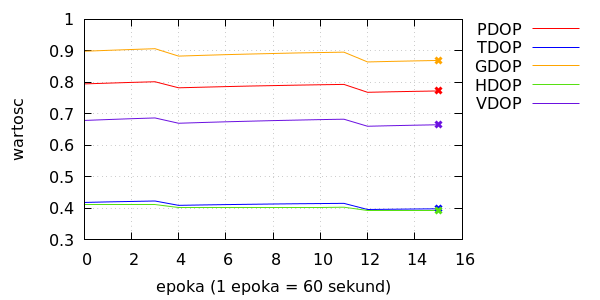
\includegraphics[width=9cm]{test.png}
\centering
\end{figure}
\newline zeby powstal wykres dop, musi wystapic przynajmniej jedna epoka w ktorej liczba widocznych satelitow bedzie wieksza badz rowna 4. dla epok w ktorych liczba widocznych satelitow byla mniejsza program nie bedzie w stanie rozwiazac mnozenia macierzy ATA. epoki takie beda wowczas pustymi obszarami na wykresie. przy wyborze mniej niz czterech satelitow, wykres dop nigdy nie powstanie. kolejny z wykresow, skyplot, pozwala na zorientowanie sie w polozeniu satelit wzgledem punktu obserwacji
\begin{figure}[h]
\caption{SKYPLOT GPS 2023-02-23 00:00+30:00}
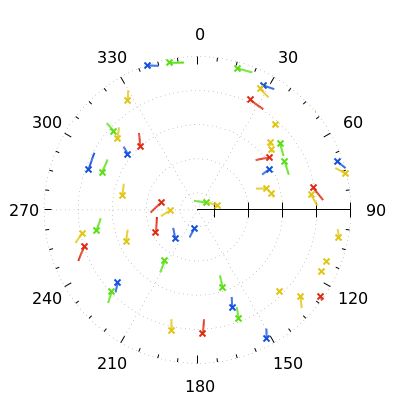
\includegraphics[width=7cm]{skyplot.png}
\centering
\end{figure}
\newline dodatkowo program generuje prosty wykres liczby widocznych satelitow w zaleznosci od czasu
\begin{figure}[h]
\caption{Widocznosc BEIDOU 2023-02-23 00+12:00:00}
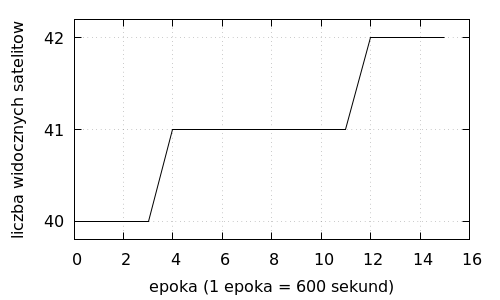
\includegraphics[width=8cm]{visible.png}
\centering
\end{figure}
\newline polaczenie danych widocznych na wszystkich wygenerowanych wykresach wystarcza do takiego dobrania czasu wykonywania pomiarow, ktory pozwoli na uzyskanie najwiekszej dokladnosci. w procesie tworzenia programu (a konkretnie - planowania wizualizacji) probowano wprowadzic wiele roznych rozwiazan z ktorych wiekszosc nie trafila do jego ostatecznej wersji. czesc eksperymentalnych wizualizacji (w tym np animacje gif z ktorych zrezygnowano przez zbyt duze skomplikowanie kodu oraz niska przejrzystosc takiegoz wykresu) mozna znalezc w zalacznikach do sprawozdania.

\section{Instrukcja obslugi}
Uzytkownik, wywolujac program z linii komend musi zaopatrzyc go w liste parametrow niezbednych do poprawnego dzialania.:
\begin{center}
\begin{tabular}{|c|c|}
\hline
     Parametr & Format  \\
\hline
     Almanach & str\(<\)path\(>\) \\
\hline
     Epoka 0 & str\(<\)YYYY-MM-DD-hh-mm-ss\(>\) \\
\hline
     Epoka 1 & str\(<\)YYYY-MM-DD-hh-mm-ss\(>\) \\
\hline
     Interwal & int[s] \\
\hline
     \(\phi\) odbiornika & float[deg] \\
\hline
     \(\lambda\) odbiornika & float[deg] \\
\hline
     \(h\) odbiornika & float[m] \\
\hline
     maska pomiaru & float[deg] \\
\hline
     satelity & -\hspace{0.02cm}- ... \\
\hline
\end{tabular}
\end{center}
parametr 'satelity' nie jest wymagany, jednak daje uzytkownikowi mozliwosc sprecyzowania tego, ktorych satelitow uzywa przy pomiarze. mozliwe jest zaznaczanie pojedynczych satelitow, badz calych systemow. do oznaczenia pojedynczego satelity wykorzystywany jest format trimble, wykorzystujacy dwu-, trzy- cyfrowe kody do identyfikacji satelitow.
\begin{center}
\begin{tabular}{|c|c|}
\hline
     ID & System \\
\hline
     1..37 & GPS \\
\hline
     38..64 & GLONASS \\
\hline
     111..118 & QZSS \\
\hline
     201..263 & Galileo \\
\hline
     264..283 & Beidou \\
\hline
\end{tabular}
\end{center}
do oznaczenia calych systemow uzytkownik jako parametr satelity podaje ich nazwy drukowanymi literami (np. GALILEO).
\section{Kompilacja}
Program nie korzysta z bibliotek zewnetrznych, zatem skompilowac mozna go z wykorzystaniem najbardziej podstawowej komendy kompilatora GPP:

\verb|g++ main.cpp -O3 -o gnssplanning| \\
a nastepnie umiescic plik binarny w folderze /bin aby byl on dostepny w calym systemie operacyjnym.

\verb|sudo mv gnssplanning /bin/gnssplanning| \\
do wykonywania wykresow program wymaga zainstalowanego narzedzia GNUPLOT w wersji 5.0+. Mozna je zainstalowac korzystajac z menadzera apt.

\verb|sudo apt install gnuplot|

\end{document}